\documentclass[border=10pt]{standalone}

\usepackage{tikz}
\usepackage{tikzsymbols}
\usetikzlibrary{calc,patterns,shapes.geometric}

\def\centerarc[#1](#2)(#3:#4:#5){\draw[#1] ($(#2)+({#5*cos(#3)},{#5*sin(#3)})$) arc (#3:#4:#5);}

\begin{document}
	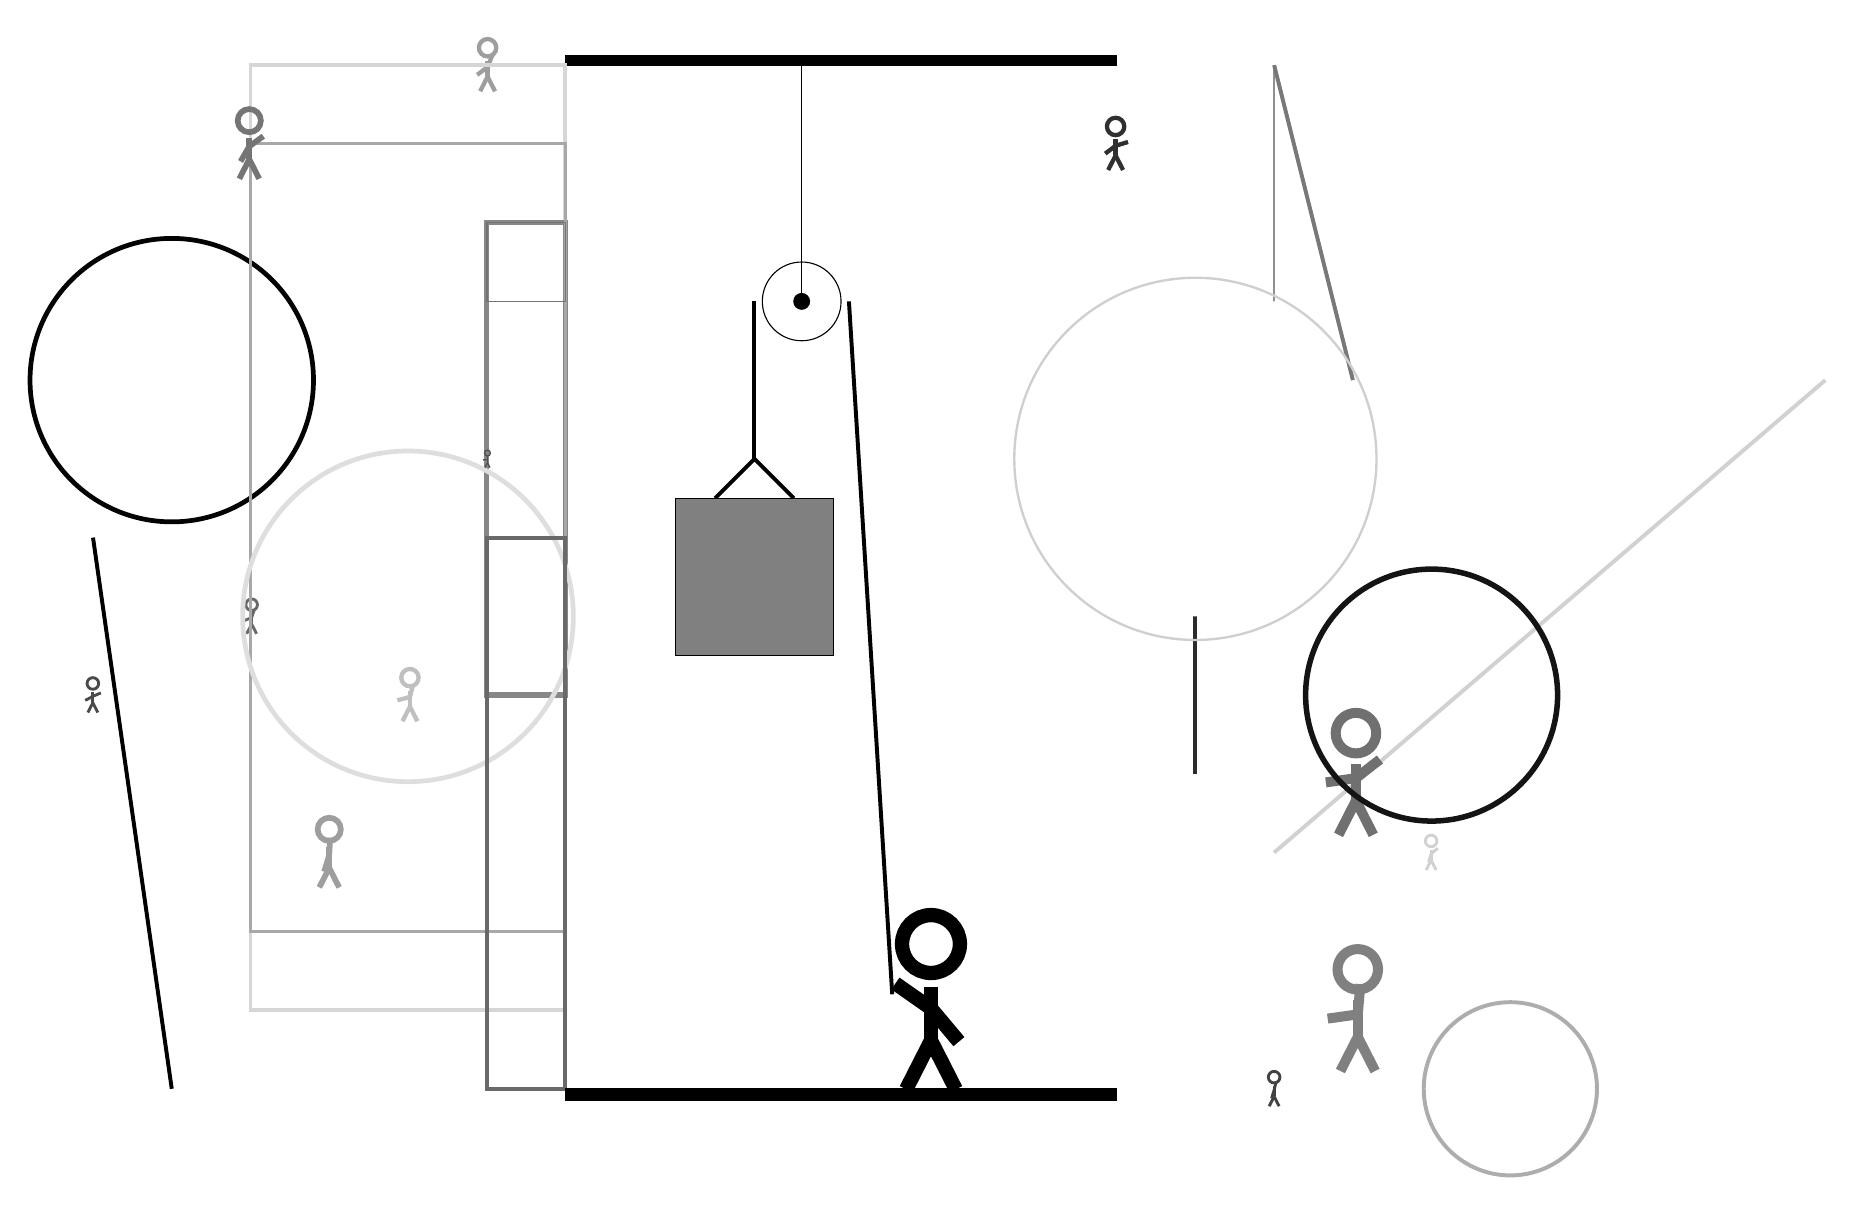
\begin{tikzpicture}
		%%%%% START %%%%%
		
		\draw[fill=black] (-2, 10) rectangle (5, 10.125);
		
		\draw (1, 7) circle (0.5);
		\draw[fill=black] (1, 7) circle (0.1);
		\draw (1, 10) -- (1, 7);
		
		\draw[line width=0.5mm] (-0.1, 4.5) -- (0.4, 5.0) -- (0.9, 4.5);
		\draw[fill=black!50] (-0.6, 4.5) rectangle (1.4, 2.5);
		
		\draw[line width=0.5mm] (0.4, 7) -- (0.4, 5.0);
		\centerarc[line width=0.5mm](1, 7)(0:180:0.6);
		\draw[line width=0.5mm](1.6, 7) -- (2.15, -1.8);
		
		\node at (2.6, -1.9) {\Strichmaxerl[10][-35][-50]};
		
		\node[line width=0.4mm, color=black!38] at (-3, 10) {\Strichmaxerl[3][37][68]};
		
		\node[line width=0.5mm, color=black!25] at (-4, 2) {\Strichmaxerl[3][15][76]};
		\draw[line width=0.5mm, color=black!18](7, 0) -- (14, 6);
		\draw[line width=0.5mm, color=black!83] (6, 1) rectangle (6, 3);
		
		\node[line width=0.7mm, color=black!38] at (-5, 0) {\Strichmaxerl[4][73][87]};
		\draw[line width=0.5mm, color=black!100](-7, -3) -- (-8, 4);
		\draw [line width=0.6mm, color=black!99](-7, 6) circle (1.8);
		
		\draw [line width=0.5mm, color=black!32](10, -3) circle (1.1);
		\draw[line width=0.5mm, color=black!16] (-2, -2) rectangle (-6, 10);
		\draw[line width=0.3mm, color=black!44] (7, 7) rectangle (7, 10);
		\draw[line width=0.7mm, color=black!47] (-3, 8) rectangle (-2, 2);
		\node[line width=0.6mm, color=black!81] at (5, 9) {\Strichmaxerl[3][37][17]};
		\node[line width=0.7mm, color=black!59] at (-6, 3) {\Strichmaxerl[2][22][71]};
		
		\draw[line width=0.4mm, color=black!34] (-2, 9) rectangle (-6, -1);
		\node[line width=0.3mm, color=black!18] at (9, 0) {\Strichmaxerl[2][73][39]};
		\draw [line width=0.6mm, color=black!13](-4, 3) circle (2.1);
		
		\node[line width=0.4mm, color=black!50] at (8, -2) {\Strichmaxerl[7][8][85]};
		\draw[line width=0.2mm, color=black!55] (-3, 8) rectangle (-2, 7);
		\node[line width=0.7mm, color=black!74] at (7, -3) {\Strichmaxerl[2][73][76]};
		\node[line width=0.7mm, color=black!56] at (8, 1) {\Strichmaxerl[7][8][38]};
		\draw [line width=0.7mm, color=black!92](9, 2) circle (1.6);
		
		\node[line width=0.4mm, color=black!71] at (-8, 2) {\Strichmaxerl[2][28][23]};
		\node[line width=0.2mm, color=black!68] at (-3, 5) {\Strichmaxerl[1][6][90]};
		\draw[line width=0.5mm, color=black!59] (-3, -3) rectangle (-2, 4);
		\draw[line width=0.5mm, color=black!53](7, 10) -- (8, 6);
		
		\node[line width=0.6mm, color=black!54] at (-6, 9) {\Strichmaxerl[4][60][36]};
		\draw [line width=0.3mm, color=black!19](6, 5) circle (2.3);
		
		\draw[fill=black] (-2, -3) rectangle (5, -3.15);
		
		%%%%% END %%%%%
	\end{tikzpicture}
\end{document}